\section{Related Work}
\label{sec:related}

This section outlines the foundational literature and methodological advancements that form the basis of our project.

\paragraph{Semantic Correspondence and Benchmarks.}
The development of dense semantic correspondence models relies heavily on robust benchmarks. \textbf{SPair-71k}~\cite{min2019spair} serves as the standard dataset for this task, featuring extreme intra-class variations in scale, viewpoint, and occlusion levels. 

\begin{figure}[ht]
    \centering
    \includegraphics[width=\columnwidth]{img/spair_examples.png}
    \caption{Examples from the SPair-71k benchmark illustrating extreme intra-class variations in scale, viewpoint, and occlusion.}
    \label{fig:spair_dataset}
\end{figure}

To overcome the discretization limits inherent in standard matching pipelines evaluated on such benchmarks, recent approaches have introduced sub-pixel refinement techniques, notably the \textit{Windowed Soft-Argmax}~\cite{zhang2024telling}.

\paragraph{Visual Foundation Models (VFMs).}
Large-scale pre-trained models provide dense feature representations that are highly effective for zero-shot matching:
\begin{itemize}
    \item \textbf{DINO Family:} Leveraging the emergent properties of Vision Transformers (ViTs)~\cite{caron2021emerging}, \textbf{DINOv2}~\cite{oquab2023dinov2} and \textbf{DINOv3}~\cite{simeoni2025dinov3} extract highly robust, unsupervised semantic features.
    \item \textbf{Segment Anything Model (SAM):}~\cite{kirillov2023segment} Trained extensively on masks, SAM provides exceptional spatial and part-to-whole decomposition, acting as a structural complement to purely semantic models.
\end{itemize}

\paragraph{Diffusion Features.}
Alongside ViTs, intermediate features extracted from generative diffusion models (e.g., Stable Diffusion) exhibit emergent geometric correspondence capabilities~\cite{tang2023emergent}. These geometry-aware representations achieve state-of-the-art zero-shot performance when complementarily fused with DINO's semantic features~\cite{zhang2023tale}.

\paragraph{Parameter-Efficient Fine-Tuning (PEFT).}
To perform supervised adaptation (e.g., light fine-tuning) without updating the entire backbone, PEFT techniques are employed:
\begin{itemize}
    \item \textbf{LoRA}~\cite{hu2022lora}: Injects trainable low-rank matrices into the Transformer blocks to drastically reduce computational overhead.
    \item \textbf{AdaptFormer}~\cite{chen2022adaptformer} and \textbf{Adapters}~\cite{houlsby2019parameter}: Insert parallel or sequential trainable bottleneck modules to efficiently adapt pre-trained models to downstream tasks.
\end{itemize}

\begin{figure}[ht]
    \centering
    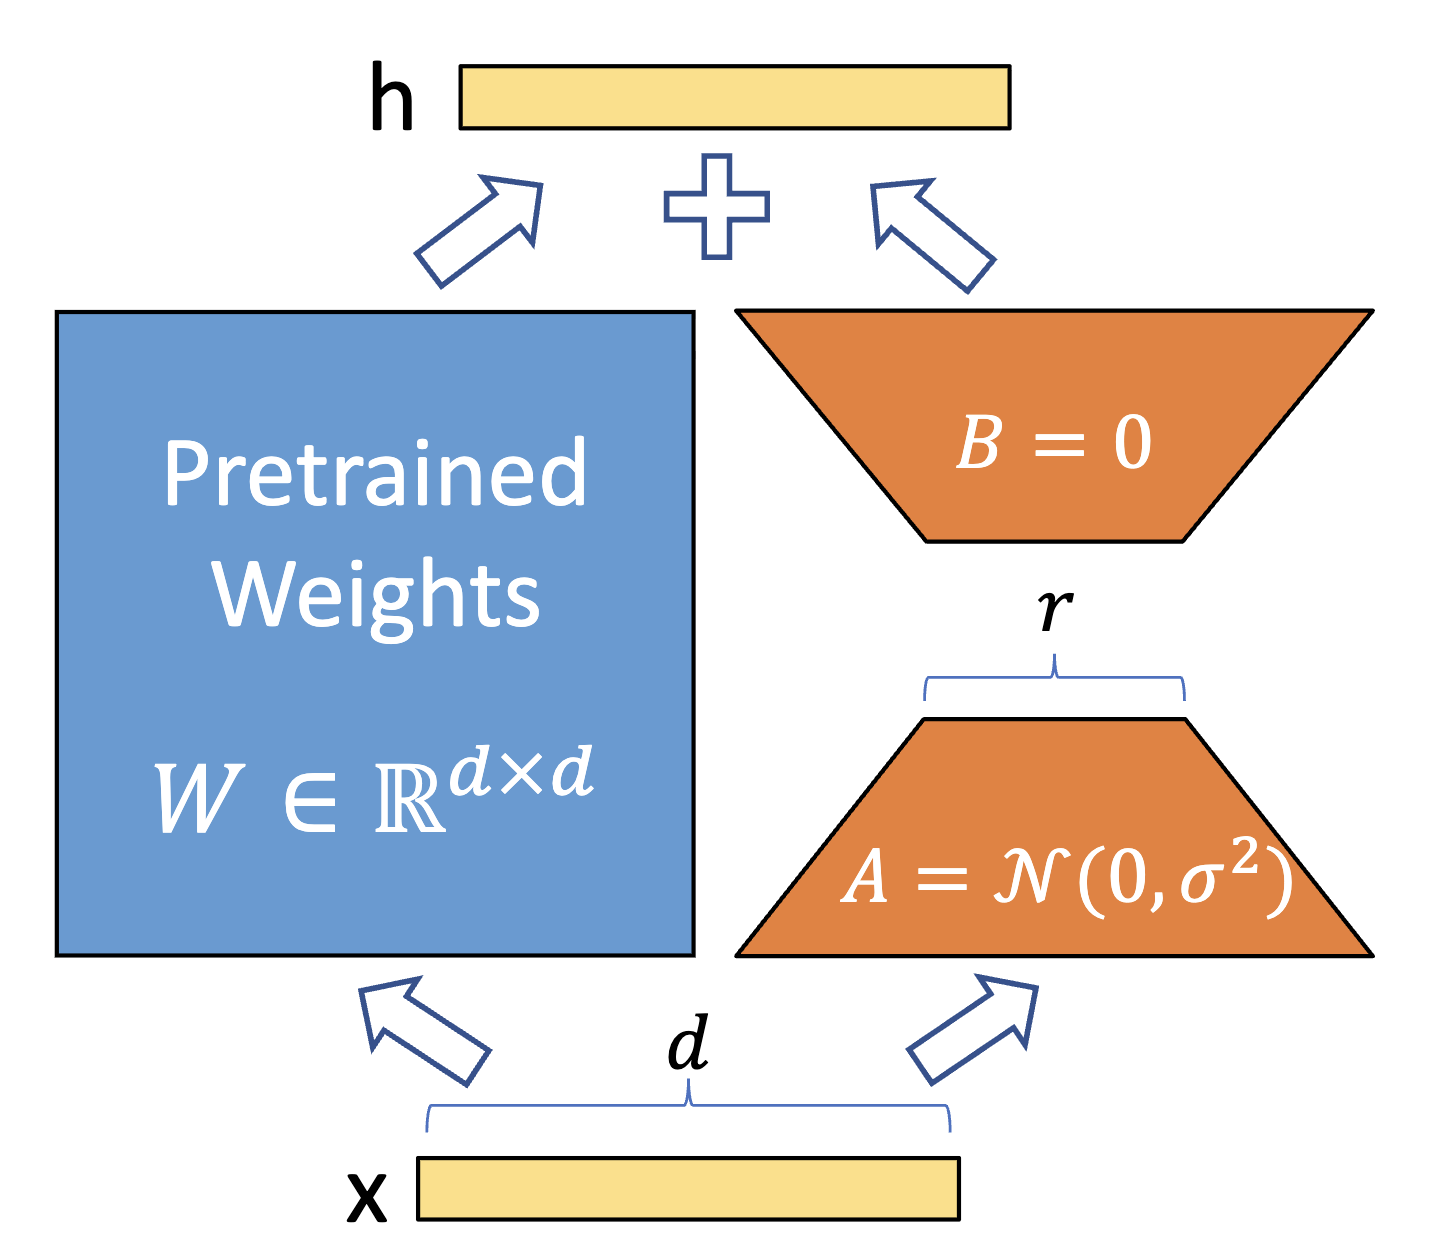
\includegraphics[width=0.6\columnwidth]{img/lora_architecture.png}
    \caption{Conceptual diagram of Parameter-Efficient Fine-Tuning (PEFT). The frozen pre-trained weights are bypassed by trainable low-rank matrices (LoRA) or parallel bottleneck modules (AdaptFormer).}
    \label{fig:peft_architecture}
\end{figure}